\subsection{Osservazione qualitativa degli andamenti}

\begin{figure}[h!]
    \centering
    \includegraphics[width=1\textwidth]{../figs/tensione-tempo.pdf}
    \caption{\emph{I grafici mostrano gli andamenti della tensione ai capi dei vari componenti quando il generatore
    oscilla ad una frequenza di $f=16kHz$ e di $f=22kHz$; questi sono valori prossimi a quelli che definiscono la banda del filtro.}}
    \label{fig:tensione-tempo}
\end{figure}


Una volta realizzato il circuito, ne è stato valutato il comportamento qualitativo. A tal proposito si è valutato visivamente
l'andamento temporale delle differenze di potenziale, a frequenza costante, sui vari elementi circuitali mediante
l'utilizzo dell'oscilloscopio digitale disponibile in laboratorio.

In secondo luogo, per una valutazione a posteriori, sono stati raccolti tali dati tramite la DAQ configurata.
In figura \ref{fig:tensione-tempo} sono mostrati tali andamenti per due valori significativi di $f$ in quanto vicini ai
valori di taglio della frequenza, caratteristici di questo circuito.
L'ampiezza dei segnali sui vari componenti, così come lo sfasamento, è consistente con il modello atteso.
%Dal secondo
%grafico si nota come $V_R$ sia leggermente sfasato rispetto a $V_{gen}$, in accordo con quanto ci si aspetta appena
%dopo il fenomeno della risonanza.


%%%%%%%%%%%%%%%%%%%%%%%%%%%%%%%%%%%%%%%%%%%%%%%%%%%%%%%%%%%%%%%%%%%%%%%%%%%%%%%%%%%%%%%%%%%%%%%%%
%%%%%%%%%%%%%%%%%%%%%%%%%%%%%%%%%%%%%%%%%%%%%%%%%%%%%%%%%%%%%%%%%%%%%%%%%%%%%%%%%%%%%%%%%%%%%%%%%
%%%%%%%%%%%%%%%%%%%%%%%%%%%%%%%%%%%%%%%%%%%%%%%%%%%%%%%%%%%%%%%%%%%%%%%%%%%%%%%%%%%%%%%%%%%%%%%%%
\subsection{Analisi delle ampiezze}

Quella che segue è l'analisi della risposta in frequenza del circuito.
È stato effettuato uno sweep in frequenza ad intervalli di $50Hz$ in un range di estremi $6kHz$ e $35kHz$, raccogliendo
$500$ campioni con un sample rate di $250000$ campioni al secondo.
I dati relativi alle ampiezza della tensione ai capi dei vari elementi sono visibili in Figura \ref{fig:ampiezzeRLC}
assieme ai fit realizzati secondo i modelli ipotizzati.
Non conoscendo in maniera precisa il funzionamento del subVI ``Extract singleton information'', che ha fornito le misurazioni
di ampiezze e fasi, è stato scelto di stimare le incertezze su tali dati tramite il rumore di fondo. È stata quindi
calcolata la deviazione standard delle misure associate all’ampiezza della tensione agli estremi, che sono posti
come costanti, ottenendo $\sigma = 3.9 \times 10^{-3} Hz$.
\begin{figure}[h]
    \centering
    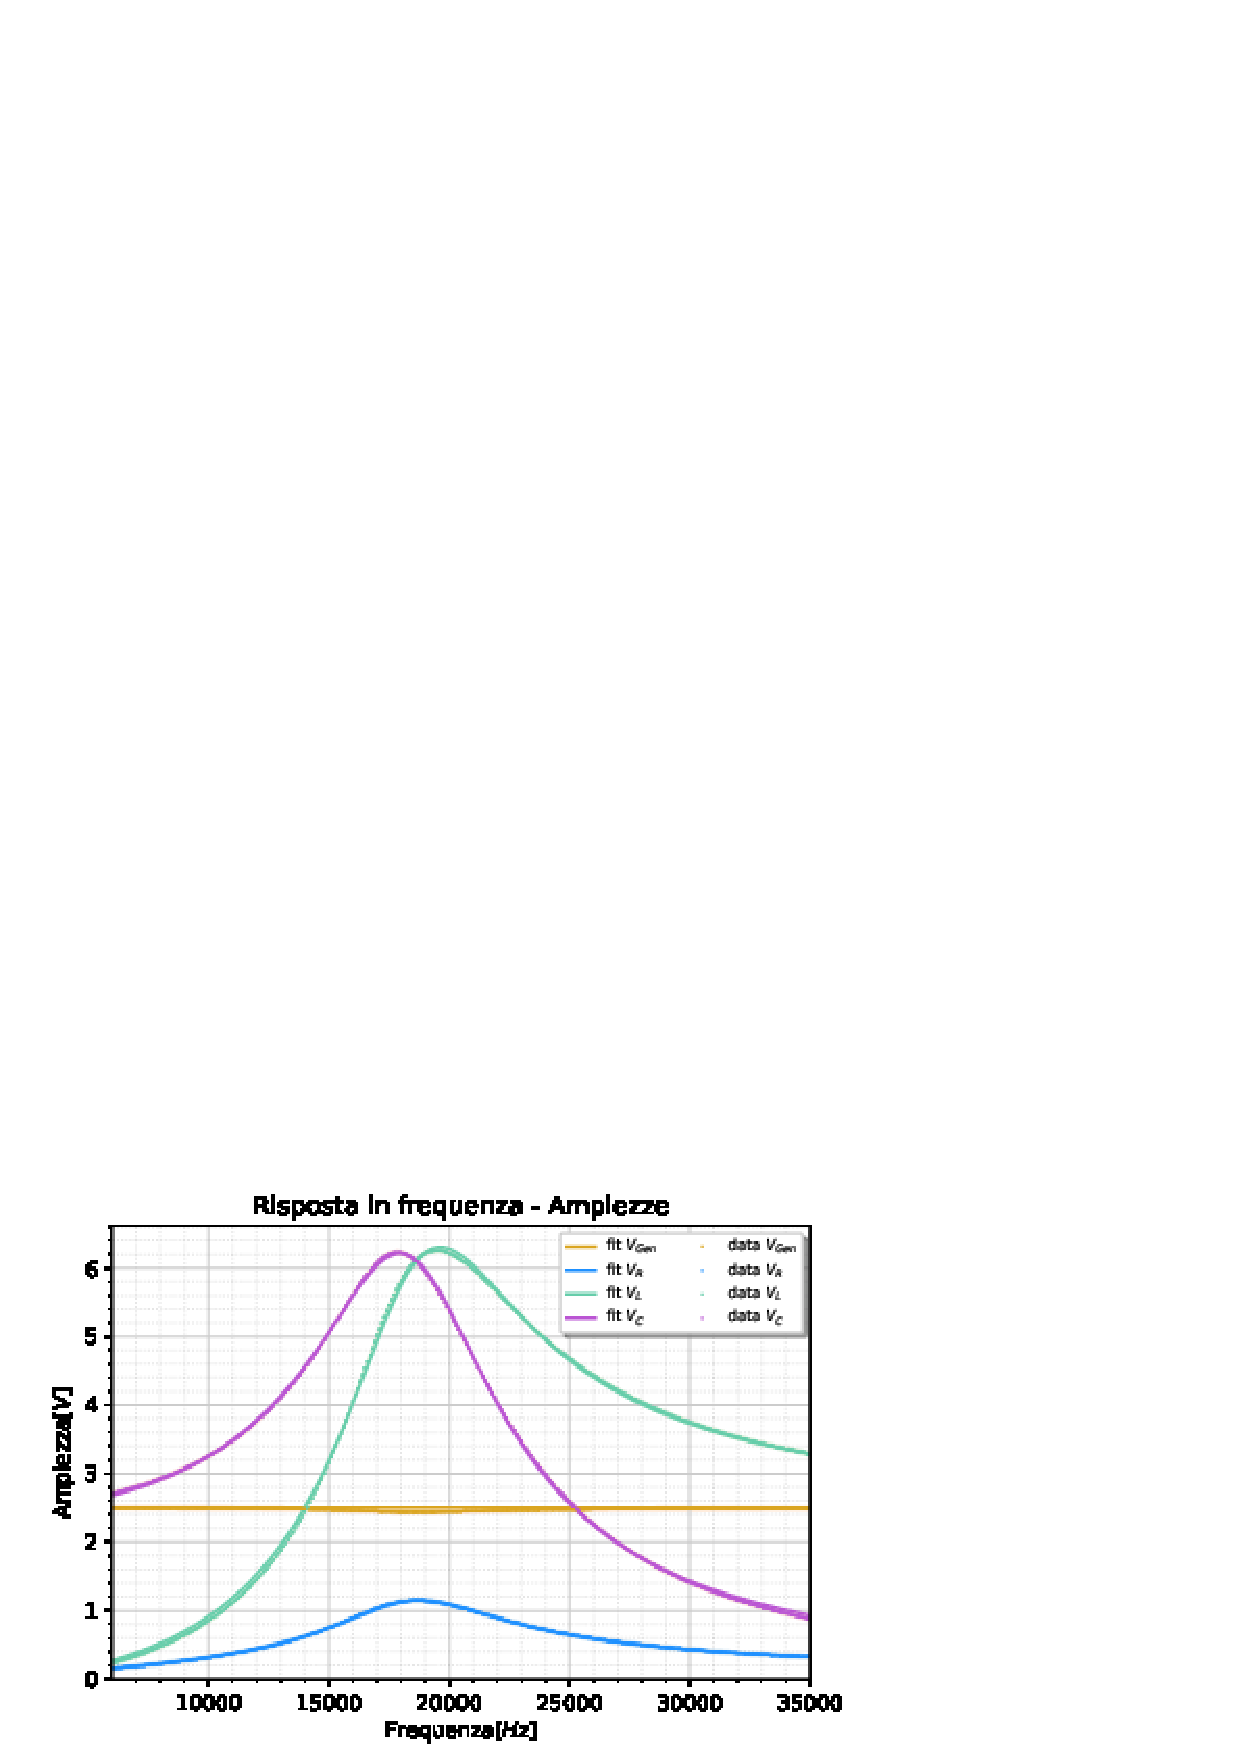
\includegraphics[width=.8\textwidth]{../figs/Risposta-in-frequenza-ampiezze.pdf}
    \caption{\emph{Andamento dell’ampiezza della tensione sui componenti del circuito al variare
    della frequenza del generatore con sovrapposte relative curve best-fit. Le incertezze sono state
    rappresentate con bande continue a causa della elevata densità di valori.}}
    \label{fig:ampiezzeRLC}
\end{figure}

Gli andamenti attesi per le varie ampiezze della tensione sono i seguenti(vedi Appendice):

\begin{equation}\label{eq:amp-V_R}
    V_R = \frac{R_rV_0}{\sqrt{ R_{tot}^2 +{ \left(\omega L - \frac{1}{\omega C}\right)}^2}}
\end{equation}
\begin{equation}
    V_L = \frac{\omega L V_0}{\sqrt{R_{tot}^2+{ \left(\omega L - \frac{1}{\omega C}\right)}^2}}
\end{equation}
\begin{equation}
    V_C = \frac{\frac{V_0}{\omega C}}{\sqrt{R_{tot}^2+{ \left(\omega L - \frac{1}{\omega C}\right)}^2}}
\end{equation}
dove $\omega$ rappresenta la pulsazione del generatore e $R_{tot}$ rappresenta la resistenza totale che si opponequicl al
fluire della corrente.



Da una prima analisi dei dati è emerso l'andamento caratteristico del filtro, con le ampiezze massimizzate
in corrispondenza di un valore specifico di frequenza.

Osservando qualitativamente il grafico, si nota una leggera diminuzione dell’ampiezza della tensione che oscilla nel filtro
per valori vicini alla frequenza di risonanza stimata. Responsabile di questo effetto è la resistenza interna del generatore
che provoca una caduta di potenziale tanto maggiore quanto lo è la corrente, che risulta essere massima proprio in
condizioni di risonanza.
 Dai fit sono emersi valori del $\tilde{\chi}^2$ piuttosto elevati; ciò è dovuto ad una sottostima dell'incertezza sui
valori di ampiezza di $V$. Pertanto, si è scelto di utilizzare come indice della goodness-of-fit
il cosiddetto coefficiente di determinazione $R^2$.
Il fit più significativo è risultato essere quello dell'ampiezza di $V_R$, mostrato in Figura \ref{fig:ampiezzeR}, con
un valore di $R^2 = 0.99946$. Da tale fit i valori dei componenti risultano essere $R_r = (1011.8 \pm 7.2) \Omega$,
$L = (4.705 \pm 0.017) \times 10^{-2}$ e $C = (1.500 \pm 0.005)\times 10^{-9}$ F. Si è scelto, inoltre, di utilizzare le
``incertezze standard'' calcolate come
\[
    \delta p_k = \sqrt{\tilde{\chi}^2 C_{kk}}
\]
dove $C_{kk}$ è l'elemento corrispondente al parametro $p_k$ nella diagonale della matrice di covarianza.
Una prima stima della frequenza di risonanza è stata ricavata applicando l'equazione (\ref{eq:res-pulsation}) con i
parametri ottenuti dal fit associato alla resistenza, ottenendo $f_0 = (18.95 \pm 0.05) kHz$, dove le incertezze sono
state propagate in quadratura.
\begin{figure}[h]
    \centering
    \includegraphics[width=.77\textwidth]{../figs/Risposta-in-frequenza-ampiezza-resistenza.pdf}
    \caption{\emph{Il grafico mostra in dettaglio l'ampiezza della tensione sul resistore, con sovrapposto relativo fit
        (equazione \ref{eq:amp-V_R}). Le incertezze sono rapresentate come in Figura \ref{fig:ampiezzeRLC}.}}\label{fig:ampiezzeR}
\end{figure}
In secondo luogo, studiando il massimo dell'ampiezza di $V_R$, si è stimato un range di valori centrato in
una certa frequenza $f$, che corrisponde teoricamente a quella di risonanza, per quanto detto in precedenza.
Individuato l’estremo inferiore della barra di errore relativa al punto di massimo estratto dal fit, si sono poi cercati i
punti in cui l’estremo superiore di tale barra corrispondesse a questo valore massimo.
Da tale procedura si è ottenuto un valore $f_0 = (18.80 \pm 0.28)kHz$.
La significatività di tale risultato, però, è ridotta, avendo sovrastimato l’incertezza, che è stata calcolata come il
valore medio dei due estremi citati precedentemente.

Un'anomalia, emersa dall'analisi dei dati raccolti, riguarda la stima della resistenza totale del circuito.
Tale valore risulta essere sistematicamente superiore a quello misurato inizialmente. In Appendice si analizza meglio
tale fenomeno.


%%%%%%%%%%%%%%%%%%%%%%%%%%%%%%%%%%%%%%%%%%%%%%%%%%%%%%%%%%%%%%%%%%%%%%%%%%%%%%%%%%%%%%%%%%%%%%%%%
%%%%%%%%%%%%%%%%%%%%%%%%%%%%%%%%%%%%%%%%%%%%%%%%%%%%%%%%%%%%%%%%%%%%%%%%%%%%%%%%%%%%%%%%%%%%%%%%%
%%%%%%%%%%%%%%%%%%%%%%%%%%%%%%%%%%%%%%%%%%%%%%%%%%%%%%%%%%%%%%%%%%%%%%%%%%%%%%%%%%%%%%%%%%%%%%%%%
\subsection{Analisi delle fasi}

Le funzioni che descrivono gli andamenti attesi delle fasi sono le seguenti:
 \begin{equation}\label{eq:fase_R}
     \phi_R = \arctan{\frac{1 - \omega^2 L C}{R_{tot} \omega C}}
 \end{equation}
 \begin{equation}
     \phi_L = \arctan{\frac{1 - \omega^2 L C}{R_{tot}  \omega C}} + \frac{\pi}{2}
 \end{equation}
\begin{equation}
    \phi_C = \arctan{\frac{1 - \omega^2 L C}{R_{tot}  \omega C}} - \frac{\pi}{2}
\end{equation}


\begin{figure}[h]
    \centering
    \includegraphics[width=.75\textwidth]{../figs/Risposta-in-frequenza-fasi.pdf}
    \caption{\emph{Andamento dello sfasamento della tensione sui componenti nello sweep in frequenza. Le incertezze
    sono rappresentate come bande continue per l'alta densità di valori.}}
    \label{fig:fasi}
\end{figure}

I dati sullo sfasamento della tensione sono stati raccolti in concomitanza con quelli sulle ampiezze. È stato scelto di
sottrarre ai dati sulle fasi di $R, L , C$ i corrispondenti valori di $\phi_{\text{gen}}$, in quanto quello che
si dovrebbe misurare è lo sfasamento rispetto al generatore.
In figura \ref{fig:fasi} sono visibili tali dati assieme alle curve best-fit, ottenute considerando solamente i valori
fra $10 kHz  \ \text{e} \ 25 kHz$ con un valore caratteristico di $R^2 = 0.991$. Il rumore di fondo è stato valutato in
maniera analoga a quanto fatto per le ampiezze, estraendo la deviazione standard degli sfasamenti a $f$ costante, con
$\sigma_{\phi} = 0.002$ rad.


Considerando il profilo dello sfasamento della tensione sulla resistenza, si è pensato di valutare la frequenza di risonanza
come la frequenza alla quale corrisponde una condizione di fase nulla tra $V_R$ e $V_{gen}$.
È stato ottenuto un valore di $f_0 = (19.10 \pm 0.10)kHz$ dove il range di valori è stato individuato dal rumore sulle fasi.
Alternativamente, $f_0$ può essere individuata dalla condizione di fase pari a $\frac{\pi}{2}$ tra $V_L$ e $V_{gen}$.
Con una procedura analoga a quella applicata nel caso di $V_R$, si ottiene $f_0 = (19.35 \pm 0.15)kHz$.






















